% Options for packages loaded elsewhere
\PassOptionsToPackage{unicode}{hyperref}
\PassOptionsToPackage{hyphens}{url}
\PassOptionsToPackage{dvipsnames,svgnames,x11names}{xcolor}
%
\documentclass[
  letterpaper,
  DIV=11,
  numbers=noendperiod]{scrartcl}

\usepackage{amsmath,amssymb}
\usepackage{lmodern}
\usepackage{iftex}
\ifPDFTeX
  \usepackage[T1]{fontenc}
  \usepackage[utf8]{inputenc}
  \usepackage{textcomp} % provide euro and other symbols
\else % if luatex or xetex
  \usepackage{unicode-math}
  \defaultfontfeatures{Scale=MatchLowercase}
  \defaultfontfeatures[\rmfamily]{Ligatures=TeX,Scale=1}
\fi
% Use upquote if available, for straight quotes in verbatim environments
\IfFileExists{upquote.sty}{\usepackage{upquote}}{}
\IfFileExists{microtype.sty}{% use microtype if available
  \usepackage[]{microtype}
  \UseMicrotypeSet[protrusion]{basicmath} % disable protrusion for tt fonts
}{}
\makeatletter
\@ifundefined{KOMAClassName}{% if non-KOMA class
  \IfFileExists{parskip.sty}{%
    \usepackage{parskip}
  }{% else
    \setlength{\parindent}{0pt}
    \setlength{\parskip}{6pt plus 2pt minus 1pt}}
}{% if KOMA class
  \KOMAoptions{parskip=half}}
\makeatother
\usepackage{xcolor}
\setlength{\emergencystretch}{3em} % prevent overfull lines
\setcounter{secnumdepth}{-\maxdimen} % remove section numbering
% Make \paragraph and \subparagraph free-standing
\ifx\paragraph\undefined\else
  \let\oldparagraph\paragraph
  \renewcommand{\paragraph}[1]{\oldparagraph{#1}\mbox{}}
\fi
\ifx\subparagraph\undefined\else
  \let\oldsubparagraph\subparagraph
  \renewcommand{\subparagraph}[1]{\oldsubparagraph{#1}\mbox{}}
\fi


\providecommand{\tightlist}{%
  \setlength{\itemsep}{0pt}\setlength{\parskip}{0pt}}\usepackage{longtable,booktabs,array}
\usepackage{calc} % for calculating minipage widths
% Correct order of tables after \paragraph or \subparagraph
\usepackage{etoolbox}
\makeatletter
\patchcmd\longtable{\par}{\if@noskipsec\mbox{}\fi\par}{}{}
\makeatother
% Allow footnotes in longtable head/foot
\IfFileExists{footnotehyper.sty}{\usepackage{footnotehyper}}{\usepackage{footnote}}
\makesavenoteenv{longtable}
\usepackage{graphicx}
\makeatletter
\def\maxwidth{\ifdim\Gin@nat@width>\linewidth\linewidth\else\Gin@nat@width\fi}
\def\maxheight{\ifdim\Gin@nat@height>\textheight\textheight\else\Gin@nat@height\fi}
\makeatother
% Scale images if necessary, so that they will not overflow the page
% margins by default, and it is still possible to overwrite the defaults
% using explicit options in \includegraphics[width, height, ...]{}
\setkeys{Gin}{width=\maxwidth,height=\maxheight,keepaspectratio}
% Set default figure placement to htbp
\makeatletter
\def\fps@figure{htbp}
\makeatother

\KOMAoption{captions}{tableheading}
\makeatletter
\makeatother
\makeatletter
\makeatother
\makeatletter
\@ifpackageloaded{caption}{}{\usepackage{caption}}
\AtBeginDocument{%
\ifdefined\contentsname
  \renewcommand*\contentsname{Table of contents}
\else
  \newcommand\contentsname{Table of contents}
\fi
\ifdefined\listfigurename
  \renewcommand*\listfigurename{List of Figures}
\else
  \newcommand\listfigurename{List of Figures}
\fi
\ifdefined\listtablename
  \renewcommand*\listtablename{List of Tables}
\else
  \newcommand\listtablename{List of Tables}
\fi
\ifdefined\figurename
  \renewcommand*\figurename{Figure}
\else
  \newcommand\figurename{Figure}
\fi
\ifdefined\tablename
  \renewcommand*\tablename{Table}
\else
  \newcommand\tablename{Table}
\fi
}
\@ifpackageloaded{float}{}{\usepackage{float}}
\floatstyle{ruled}
\@ifundefined{c@chapter}{\newfloat{codelisting}{h}{lop}}{\newfloat{codelisting}{h}{lop}[chapter]}
\floatname{codelisting}{Listing}
\newcommand*\listoflistings{\listof{codelisting}{List of Listings}}
\makeatother
\makeatletter
\@ifpackageloaded{caption}{}{\usepackage{caption}}
\@ifpackageloaded{subcaption}{}{\usepackage{subcaption}}
\makeatother
\makeatletter
\@ifpackageloaded{tcolorbox}{}{\usepackage[many]{tcolorbox}}
\makeatother
\makeatletter
\@ifundefined{shadecolor}{\definecolor{shadecolor}{rgb}{.97, .97, .97}}
\makeatother
\makeatletter
\makeatother
\ifLuaTeX
  \usepackage{selnolig}  % disable illegal ligatures
\fi
\IfFileExists{bookmark.sty}{\usepackage{bookmark}}{\usepackage{hyperref}}
\IfFileExists{xurl.sty}{\usepackage{xurl}}{} % add URL line breaks if available
\urlstyle{same} % disable monospaced font for URLs
\hypersetup{
  pdftitle={First Class},
  pdfauthor={Marguerite Butler},
  colorlinks=true,
  linkcolor={blue},
  filecolor={Maroon},
  citecolor={Blue},
  urlcolor={Blue},
  pdfcreator={LaTeX via pandoc}}

\title{First Class}
\author{Marguerite Butler}
\date{}

\begin{document}
\maketitle
\ifdefined\Shaded\renewenvironment{Shaded}{\begin{tcolorbox}[enhanced, breakable, interior hidden, borderline west={3pt}{0pt}{shadecolor}, boxrule=0pt, sharp corners, frame hidden]}{\end{tcolorbox}}\fi

\renewcommand*\contentsname{Table of contents}
{
\hypersetup{linkcolor=}
\setcounter{tocdepth}{3}
\tableofcontents
}
\hypertarget{data-science}{%
\subsection{Data Science}\label{data-science}}

\hypertarget{from-r-for-data-science-2e-by-hadley-wickam-garrett-grolemund-and-mine-uxe7etinkaya-rundel}{%
\paragraph{\texorpdfstring{From \href{https://r4ds.hadley.nz/}{R for
Data Science 2e} by Hadley Wickam, Garrett Grolemund, and Mine
Çetinkaya-Rundel}{From R for Data Science 2e by Hadley Wickam, Garrett Grolemund, and Mine Çetinkaya-Rundel}}\label{from-r-for-data-science-2e-by-hadley-wickam-garrett-grolemund-and-mine-uxe7etinkaya-rundel}}

\begin{figure}

{\centering 

\href{https://r4ds.hadley.nz/whole-game.html}{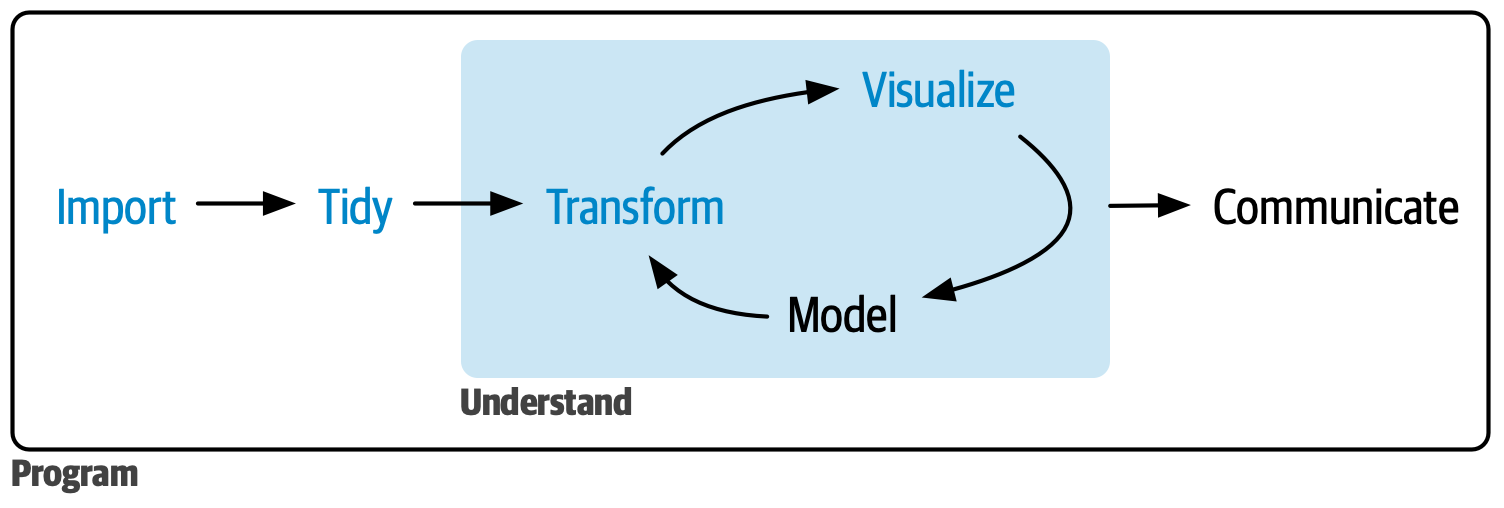
\includegraphics{whole-game.png}}

}

\end{figure}

\begin{itemize}
\tightlist
\item
  Question -\textgreater{} Gather Data -\textgreater{} Design
\item
  Observe -\textgreater{} Record Data -\textgreater{} Data Table
\item
  Document -\textgreater{} Comment (annotate)
\item
  Project -\textgreater{} Version Control -\textgreater{} Share
\end{itemize}

\hypertarget{learning-r---a-first-session}{%
\subsection{Learning R - A first
session}\label{learning-r---a-first-session}}

\begin{itemize}
\tightlist
\item
  Think about how R works as you try out commands
\item
  \url{https://www.r-project.org} Go to manuals, click on \textbf{An
  Introduction to R}
\item
  Follow Section 2.1
\item
  input -\textgreater{} R -\textgreater{} output
\item
  What came out? What does it tell you about the rules R follows?
\item
  Computers only do \textbf{Exactly} what you tell them to do
\item
  Jump to Appendix A - letʻs try to understand some rules of R together
\end{itemize}

\hypertarget{goals}{%
\subsection{Goals}\label{goals}}

\begin{itemize}
\tightlist
\item
  Creativity
\item
  Accuracy
\item
  Authority
\item
  Repeatability
\item
  Communication

  \begin{itemize}
  \tightlist
  \item
    Ease of dissemination to other researchers
  \item
    Show me, donʻt tell me
  \end{itemize}
\end{itemize}

\hypertarget{tools}{%
\subsection{Tools}\label{tools}}

\begin{itemize}
\tightlist
\item
  Our senses
\item
  Notebooks and Pens
\item
  Excel
\item
  Command Line (UNIX/ Windows/ File Commands in your operating system)
\item
  R
\item
  Git/GitHub
\item
  Quarto/Rmarkdown
\item
  and many more\ldots{}
\end{itemize}

\hypertarget{data-science-1}{%
\subsection{Data Science}\label{data-science-1}}

\begin{figure}

{\centering 

\href{https://r4ds.hadley.nz/whole-game.html}{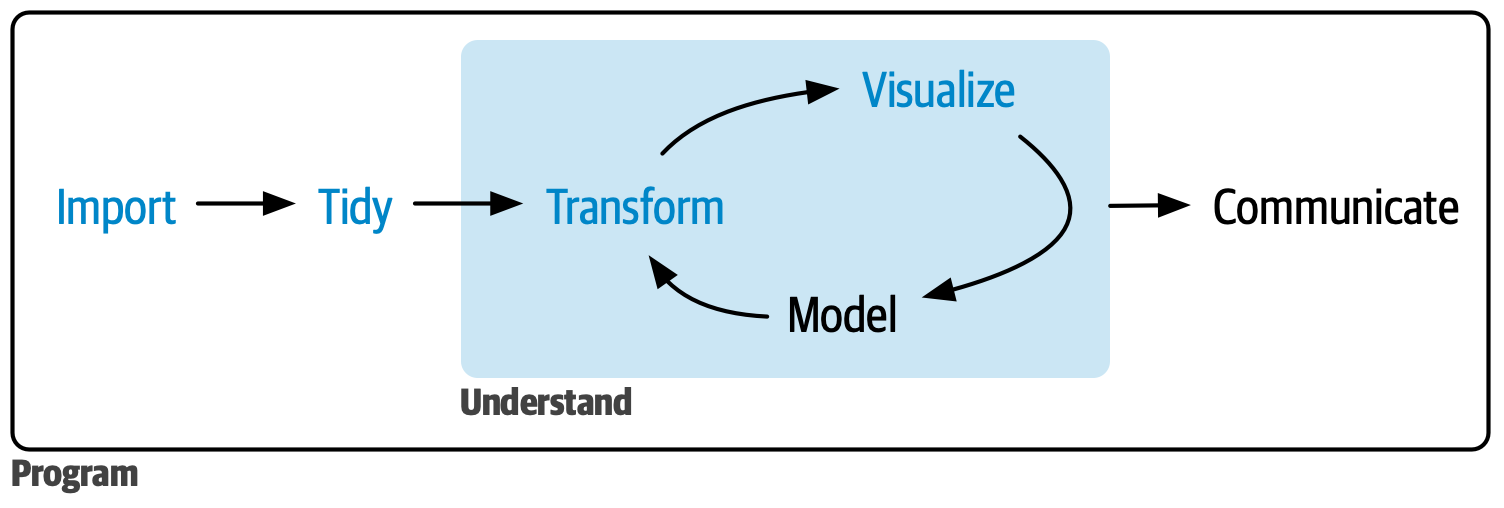
\includegraphics{whole-game.png}}

}

\end{figure}

\begin{longtable}[]{@{}ll@{}}
\toprule()
Need & Tools \\
\midrule()
\endhead
Observe -\textgreater{} Record Data -\textgreater{} Data Table &
\emph{Notebooks} \\
Document -\textgreater{} Comment (annotate) & \emph{R} \\
Project -\textgreater{} Version Control -\textgreater{} Share &
\emph{Git/GitHub} \\
Communicate & \emph{R/ Quarto} \\
\bottomrule()
\end{longtable}

\hypertarget{software}{%
\subsection{Software}\label{software}}

\begin{itemize}
\tightlist
\item
  Do you have R installed and working? (R studio is optional)
\item
  For a longer walk-through here is another resource:
  \href{https://www.stephaniehicks.com/jhustatcomputing2022/posts/2022-08-30-introduction-to-r-and-rstudio/}{Introduction
  to R/Rstudio}
\item
  Git/GitHub: Please Install. Letʻs follow
  \href{https://www.stephaniehicks.com/jhustatcomputing2022/posts/2022-08-30-introduction-to-gitgithub/}{Introduction
  to Git/GitHub}
\end{itemize}



\end{document}
